%\documentclass[handout]{beamer} 
\documentclass[t,12pt,numbers,fleqn]{beamer}
%\documentclass[ignorenonframetext]{beamer}

\newif\ifquestions
%\questionstrue
\questionsfalse

\usepackage{pgfpages} 
\usepackage{hyperref}
\hypersetup{colorlinks=true,
    linkcolor=blue,
    citecolor=blue,
    filecolor=blue,
    urlcolor=blue,
    unicode=false}
\urlstyle{same}

\bibliographystyle{plain}

%\usetheme{Iimenau}

\useoutertheme{split} %so the footline can be seen, without needing pgfpages

%\pgfpagesuselayout{resize to}[letterpaper,border shrink=5mm,landscape]  %if this is uncommented, the hyperref links do not work

\mode<presentation>{}

\input{../def-beamer}

\newcommand{\topic}{22 Assurance Case}

%Title page information for 1D04 lectures slides

% Define year specific parameters - used in title page and footer

\newcommand{\season}{Fall} %use to switch between Winter and Fall
\newcommand{\instructor}{Dr.~Spencer Smith} %use to switch instructor
\newcommand{\instructSmall}{Dr.~Smith}
\newcommand{\yr}{2019}
\newcommand{\courseCode}{CAS 741, CES 741}
\newcommand{\courseTitle}{Development of Scientific Computing Software}

%\setbeamerfont{structure}{series=\bfseries}
%\usefonttheme[stillsansseriftext,stillsansserifmath]{serif}
\setbeamertemplate{navigation symbols}{} 
\setbeamertemplate{itemize item}[ball]

\title{
  {\normalsize \bf 
    \borange{\courseCode~(\courseTitle)\\ \season~\yr}}\\[2ex]
  {\Large \bf \topic}}

\author[Smith]{\instructor}

\institute{
  Faculty of Engineering,
  McMaster University}

\date{
\today
%January 2011\\
\bc
  \includegraphics[scale = 0.2, keepaspectratio]
  {../mcmaster-logo-full-color.jpg}
\ec
}

\renewcommand{\borange}[1] %orange is too hard to read
{
   \bred{#1}
}

\begin{document}

\input{../footline}

%%%%%%%%%%%%%%%%%%%%%%%%%%%%%%%%%%%%%%%%%%%%%%%%%%%%%%

\begin{frame}
\frametitle{Assurance Case}

\bi
\item Administrative details
\item Questions?
\item License and copyright
\item Assurance cases
\ei
\end{frame}

%%%%%%%%%%%%%%%%%%%%%%%%%%%%%%%%%%%%%%%%%%%%%%%%%%%%%%

\begin{frame}
\frametitle{Administrative Details}

\bi
\item Course evaluation
\bi
\item Nov 23 to Dec 7
\item \url{https://evals.mcmaster.ca}
\ei
\item GitHub issues for colleagues
\bi
\item Assigned 1 colleague (see \texttt{Repos.xlsx} in repo)
\item Provide at least 5 issues on their MIS
\item Grading as before
\item Due by Tuesday, Dec 5, 11:59 pm
\ei
\item Today is the last ``lecture''
\item Next week for presentations
\item Following Tuesday for Discussion
\ei

\end{frame}

%%%%%%%%%%%%%%%%%%%%%%%%%%%%%%%%%%%%%%%%%%%%%%%%%%%%%%

\begin{frame}
\frametitle{Administrative Details: Deadlines}
~\newline
\begin{tabular}{l l l}
\textbf{MIS} & Week 11 & Nov 29\\
\textbf{Impl.\ Present} & Week 12 & Week of Nov 27\\
\textbf{Final Documentation} & Week 13 & Dec 6\\
\end {tabular}

\end{frame}

%%%%%%%%%%%%%%%%%%%%%%%%%%%%%%%%%%%%%%%%%%%%%%%%%%%%%%

\begin{frame}
\frametitle{Administrative Details: Presentation Schedule}

\bi
\item {Impl.\ Present}
\bi
\item \textbf{Tuesday: Alexander S., Steven, Alexandre P.}
\item \textbf{Friday: Jason, Geneva, Yuzhi}
\ei
\item Can present anything related to the implementation
\bi
\item Code
\item Tools used
\item Testing
\item As always it is fine to show work in progress
\item Good to bring questions to the class
\ei
\ei

\end{frame}

%%%%%%%%%%%%%%%%%%%%%%%%%%%%%%%%%%%%%%%%%%%%%%%%%%%%%%

\begin{frame}
\frametitle{Final Documentation}
\begin{itemize}
\item Looking for 
\bi
\item Revision of documentation
\item Consistency between documents
\item Traceability between documents - should be able to pick a requirement and
  trace it all the way to testing
\item Effort made to address issues and comments
\item Appropriate challenge level
\ei
\item Make it easy to see changes from Rev 0
\bi
\item Specific explanation in Revision History
\item Comments in tex file
\ei
\end{itemize}
\end{frame}

%%%%%%%%%%%%%%%%%%%%%%%%%%%%%%%%%%%%%%%%%%%%%%%%%%%%%%

\begin{frame}
\frametitle{Final Documentation}
\begin{itemize}
\item Requirements Document revised and improved
\item Design Documents revised and improved
\item Test Plan revised and improved
\item Test Report
\item Source Code
\end{itemize}
\end{frame}

%%%%%%%%%%%%%%%%%%%%%%%%%%%%%%%%%%%%%%%%%%%%%%%%%%%%%%

\begin{frame}
\frametitle{Final Documentation: Source Code}
\begin{itemize}
\item Comments on ``what'' not ``how''
\item Identifiers that are consistent, distinctive, and meaningful
\item Avoidance of hard-coded constants (other than maybe 0 and 1)
\item Appropriate modularization
\item Consistent indentation
\item Explicit identification of coding standards
\item Parameters are in the same order for all functions
\item Descriptive names of source code files
\item Traceability to modules in module guide
\end{itemize}
\end{frame}

%%%%%%%%%%%%%%%%%%%%%%%%%%%%%%%%%%%%%%%%%%%%%%%%%%%%%%

\begin{frame}
\frametitle{Final Documentation}
\begin{itemize}
\item Traceability between documents
\item Look for an obvious requirement to see if it is in the requirements
  document and traceable through the other documents
\item Installability - instructions given, makefiles etc to support, means to
  validate the installation, required libraries are explicitly identified
\item Learnability - instructions to get someone started using the software
\item Robustness - can the software handle garbage inputs reasonably
\item Performance - measured if appropriate
\item Usability - measured if appropriate
\end{itemize}
\end{frame}

%%%%%%%%%%%%%%%%%%%%%%%%%%%%%%%%%%%%%%%%%%%%%%%%%%%%%%

\begin{frame}
\frametitle{Questions?}
\begin{itemize}
\item Questions about MIS documentation?
\item Questions about implementation presentations?
\end{itemize}
\end{frame}

%%%%%%%%%%%%%%%%%%%%%%%%%%%%%%%%%%%%%%%%%%%%%%%%%%%%%%

\begin{frame}
\frametitle{No License?}

\bi
\item Can others use your work if you do not include a license?
\item \href{http://choosealicense.com/no-license/}{See this link for the answer}
\ei

\end{frame}

%%%%%%%%%%%%%%%%%%%%%%%%%%%%%%%%%%%%%%%%%%%%%%%%%%%%%%%%%%%%%%%%%%%%%%%%%%%%%

\begin{frame}
\frametitle{Copyright}

\bi
\item Your work is automatically afforded protection by copyright law
\bi
\item Your cannot infringe on someone else's copyright
\item Must be some creativity
\ei
\item Additional protection through registration with the copyright office
\item Copyright does not apply to the idea, but the expression of the idea
\item Trademarks and patents cover concepts and ideas
\item In work for hire, copyright belongs to employer
\item You can assign your copyright to someone else or a corporation
\ei

\end{frame}

%%%%%%%%%%%%%%%%%%%%%%%%%%%%%%%%%%%%%%%%%%%%%%%%%%%%%%%%%%%%%%%%%%%%%%%%%%%%%

\begin{frame}
\frametitle{Rights}

\bi
\item Owner has full and exclusive rights to control who may copy or create a
  derivative work
\item Right to sue for copyright infringement
\ei

\end{frame}

%%%%%%%%%%%%%%%%%%%%%%%%%%%%%%%%%%%%%%%%%%%%%%%%%%%%%%%%%%%%%%%%%%%%%%%%%%%%%

\begin{frame}
\frametitle{Licensing}

\bi
\item Permission to others to reproduce or distribute a work
\item Licenses are distinguished by the restrictions (conditions)
\ei

\end{frame}

%%%%%%%%%%%%%%%%%%%%%%%%%%%%%%%%%%%%%%%%%%%%%%%%%%%%%%%%%%%%%%%%%%%%%%%%%%%%%

\begin{frame}
\frametitle{Proprietary License}

\bi
\item Copyright holder retains all rights
\item Cannot copy
\item Cannot use
\item Cannot modify
\ei

\end{frame}

%%%%%%%%%%%%%%%%%%%%%%%%%%%%%%%%%%%%%%%%%%%%%%%%%%%%%%%%%%%%%%%%%%%%%%%%%%%%%

\begin{frame}
\frametitle{GNU General Public License (GPL)}

\bi
\item Can copy the software
\item Can distribute the software
\item Can charge a fee to distribute the software (which will still include the license information)
\item Can make modifications
\item Condition -- all modifications/uses are also under GPL, source
  code must be available
\item Lesser GPL allows to link to libraries, without automatically falling under
  GPL conditions
\ei

\end{frame}

%%%%%%%%%%%%%%%%%%%%%%%%%%%%%%%%%%%%%%%%%%%%%%%%%%%%%%%%%%%%%%%%%%%%%%%%%%%%%

\begin{frame}
\frametitle{GNU Questions}

\bi
\item Question 1
\bi
\item You modify some Linux source files to install Linux on your embedded
  device
\item You write software to run on this new Linux ``box''
\item What software falls under the GPL?
\item \href{http://www.softwarefreedom.org/resources/2008/compliance-guide.html}{Answer}
\ei
\item Question 2
\bi
\item You want to distribute object code compiled by gcc, where gcc is under GPL
\item Is your object code under GPL?
\item \href{https://www.gnu.org/licenses/gcc-exception-3.1-faq.en.html}{Answer}
\ei
\ei

\end{frame}

%%%%%%%%%%%%%%%%%%%%%%%%%%%%%%%%%%%%%%%%%%%%%%%%%%%%%%%%%%%%%%%%%%%%%%%%%%%%%

\begin{frame}
\frametitle{BSD and MIT}

\bi
\item Removes ``virus'' from GPL
\item Can copy, distribute, charge a fee, make modifications
\item Under the condition that you keep the license intact, credit the author
\item Not required to disclose source 
\item Use at your own risk (cannot sue)
\ei

\end{frame}

%%%%%%%%%%%%%%%%%%%%%%%%%%%%%%%%%%%%%%%%%%%%%%%%%%%%%%%%%%%%%%%%%%%%%%%%%%%%%

\begin{frame}
\frametitle{Public Domain}

\bi
\item Do what you want with the code
\item No conditions
\ei

\end{frame}

%%%%%%%%%%%%%%%%%%%%%%%%%%%%%%%%%%%%%%%%%%%%%%%%%%%%%%%%%%%%%%%%%%%%%%%%%%%%%

\begin{frame}
\frametitle{Copyright and License Related Links}

\bi
\item
  \href{http://haacked.com/archive/2006/01/24/TheDevelopersGuideToCopyrightLaw-Part1.aspx/}{Developer's
    guide to copyright law}

\item \href{https://www.smashingmagazine.com/2010/03/a-short-guide-to-open-source-and-similar-licenses/}{Summary of licenses}

\item
  \href{http://haacked.com/archive/2007/04/04/there-are-only-four-software-licenses.aspx/}{Main
    types of licenses}

\item \href{http://choosealicense.com}{Choose a license}
\item \href{http://choosealicense.com/licenses/}{Another summary}
\item \href{https://tldrlegal.com}{Plain English summaries}

\ei

\end{frame}

%%%%%%%%%%%%%%%%%%%%%%%%%%%%%%%%%%%%%%%%%%%%%%%%%%%%%%%%%%%%%%%%%%%%%%%%%%%%%

\begin{frame}
\frametitle{Assurance Cases in Scientific Computing \cite{SmithEtAl2017}}

\bi
\item Assurance cases
\bi 
\item Organized and explicit argument for correctness
\item Successfully used for safety critical systems
\ei
\item Advantages for SC
\bi
\item Engaging domain experts
\item Producing necessary and relevant documentation
\item Evidence that can be verified/replicated by a third party
\ei
\item Example of 3dfim+
\bi
\item No errors found
\item However
\bi
\item Documentation ambiguities
\item No warning about parametric statistical model
\ei
\ei
\ei

\end{frame}

%%%%%%%%%%%%%%%%%%%%%%%%%%%%%%%%%%%%%%%%%%%%%%%%%%%%%%%%%%%%%%%%%%%%%%%%%%%%%

\begin{frame}
\frametitle{Assurance Cases in SC Motivation}

\bi
\item Do we put too much trust in the quality of SCS?
\item Are enough checks and balances in place, especially for safety related
  software?
\item Problems with imposing external requirements for certification
\bi
\item External body does not have expertise
\item SCS developers dislike documentation
\ei
\item Solution -- Assurance Cases by experts
\bi
\item Experts engaged
\item Relevant documentation
\ei
\item Current techniques of development and testing still used, but arguments
  will no longer be ad hoc and incompletely documented
\ei

\end{frame}

%%%%%%%%%%%%%%%%%%%%%%%%%%%%%%%%%%%%%%%%%%%%%%%%%%%%%%%%%%%%%%%%%%%%%%%%%%%%%

\hoffset=-.45in
\begin{frame}[plain]
%\frametitle{Goal Structuring Notation}

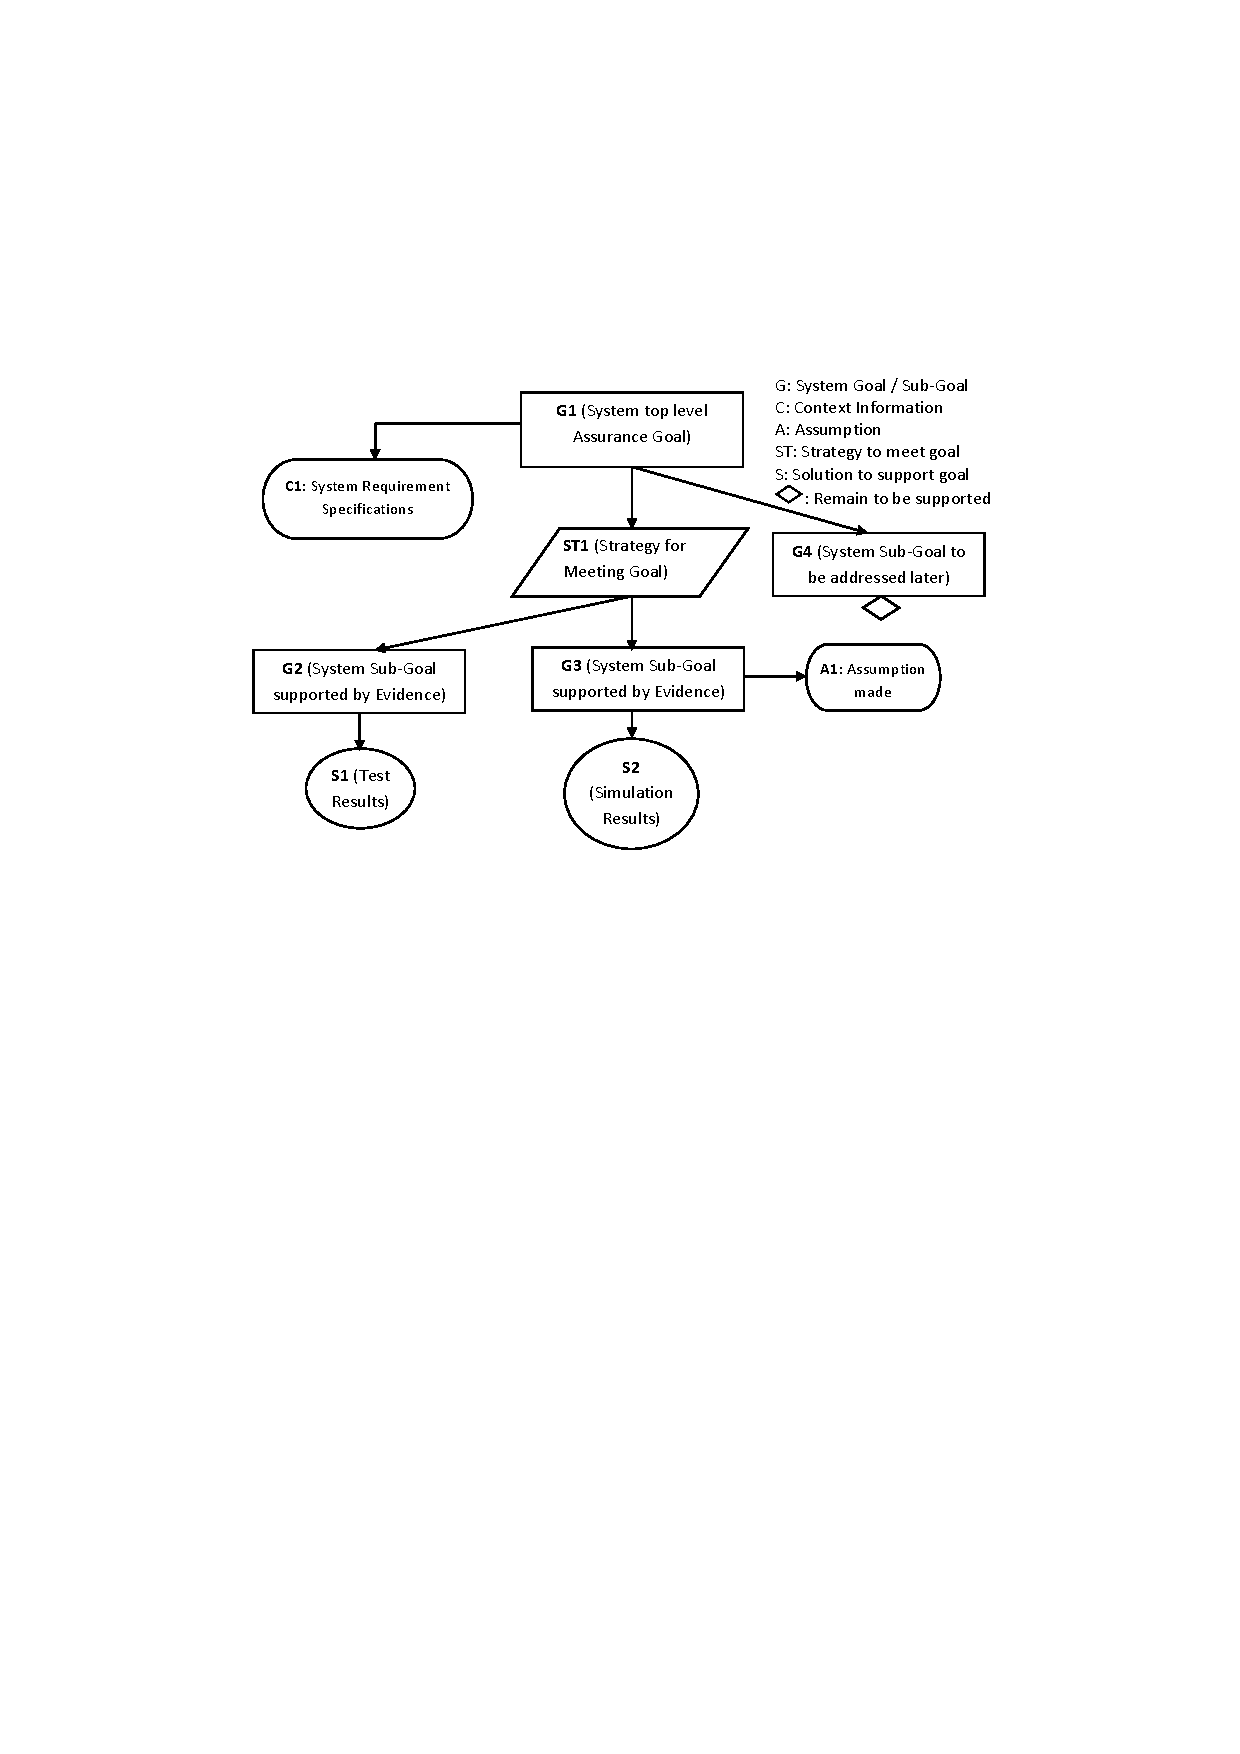
\includegraphics[width=1.19\textwidth]{../Figures/assuranceBasic.pdf}

\end{frame}
\hoffset=0in

%%%%%%%%%%%%%%%%%%%%%%%%%%%%%%%%%%%%%%%%%%%%%%%%%%%%%%%%%%%%%%%%%%%%%%%%%%%%%

\hoffset=-.2in
\begin{frame}[plain]
%\frametitle{3dfim+ Software}

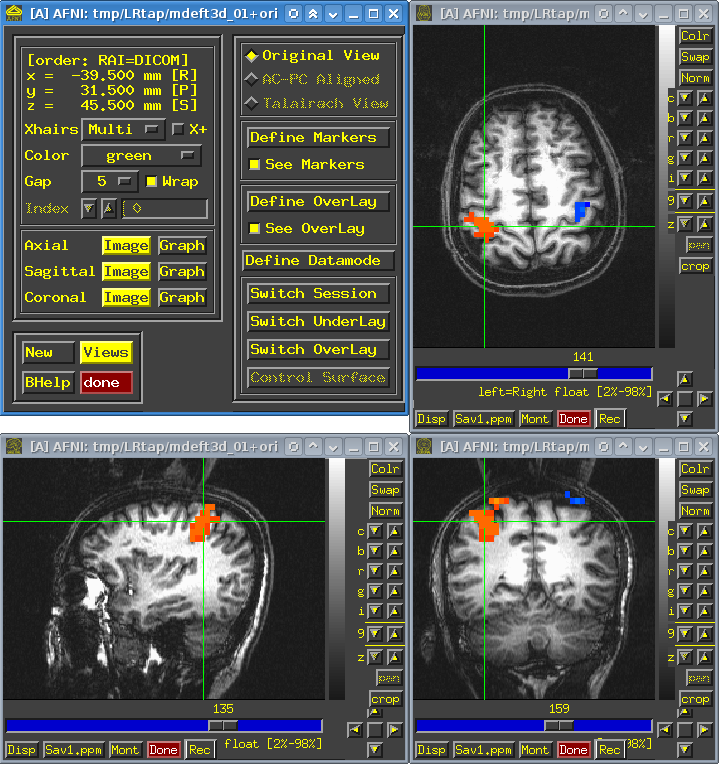
\includegraphics[width=1.\textwidth]{../Figures/AFNI_screenshot.PNG}

\end{frame}
\hoffset=0in

%%%%%%%%%%%%%%%%%%%%%%%%%%%%%%%%%%%%%%%%%%%%%%%%%%%%%%%%%%%%%%%%%%%%%%%%%%%%%

\hoffset=-.2in
\begin{frame}[plain]
%\frametitle{Correlation of One Voxel}

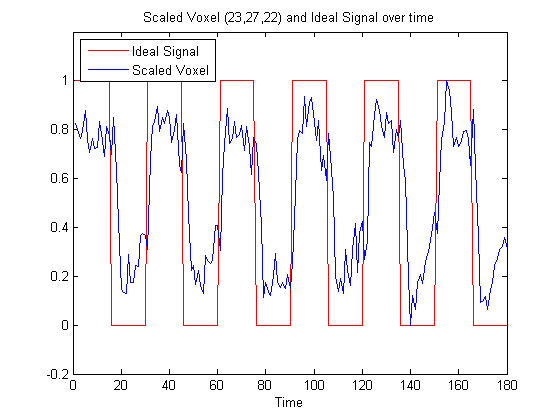
\includegraphics[width=1.\textwidth]{../Figures/scaledvoxelANDIdealsignalVStime_least.png}

\end{frame}
\hoffset=0in

%%%%%%%%%%%%%%%%%%%%%%%%%%%%%%%%%%%%%%%%%%%%%%%%%%%%%%%%%%%%%%%%%%%%%%%%%%%%%

\hoffset=-.2in
\begin{frame}[plain]
%\frametitle{Context and Assumption in Top Goal}

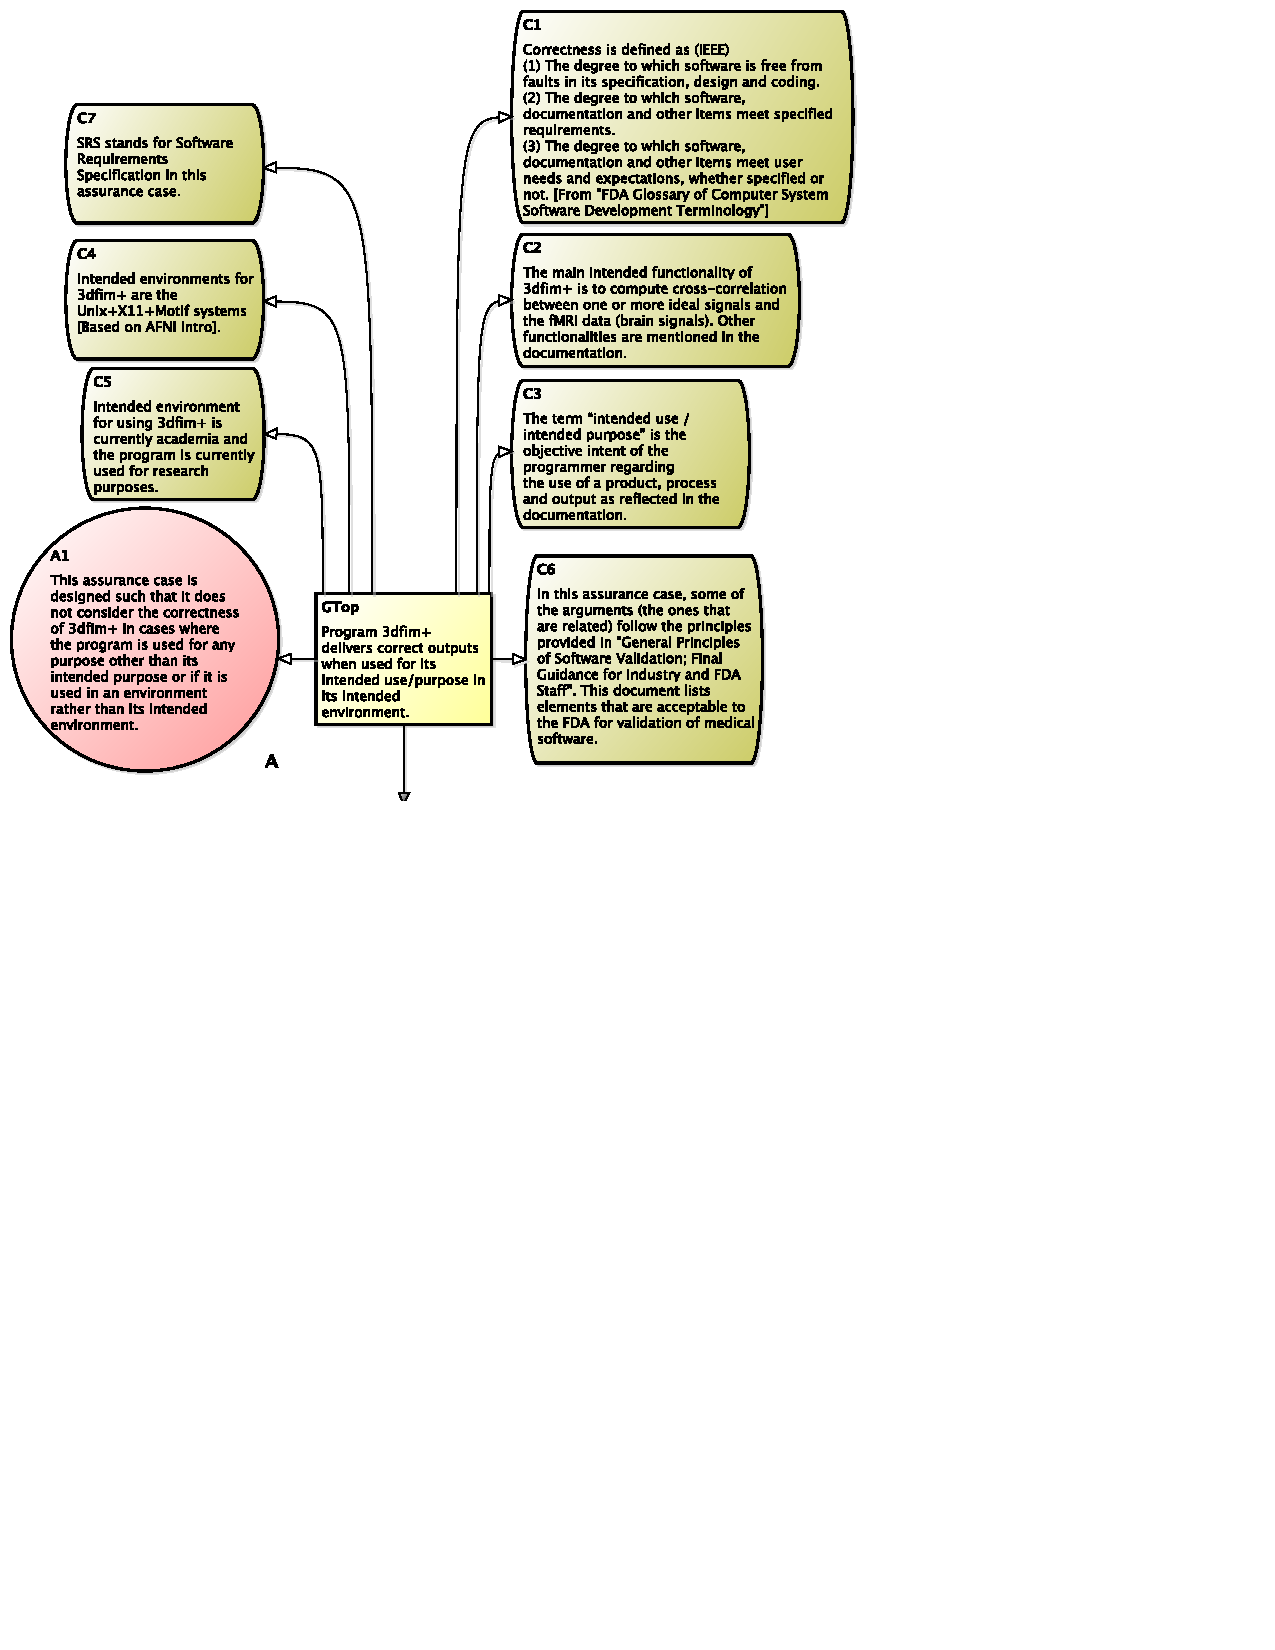
\includegraphics[width=0.95\textwidth]{../Figures/TopAC.pdf}

\end{frame}
\hoffset=0in

%%%%%%%%%%%%%%%%%%%%%%%%%%%%%%%%%%%%%%%%%%%%%%%%%%%%%%%%%%%%%%%%%%%%%%%%%%%%%

\hoffset=-.27in
\begin{frame}[plain]
%\frametitle{Top Goal}

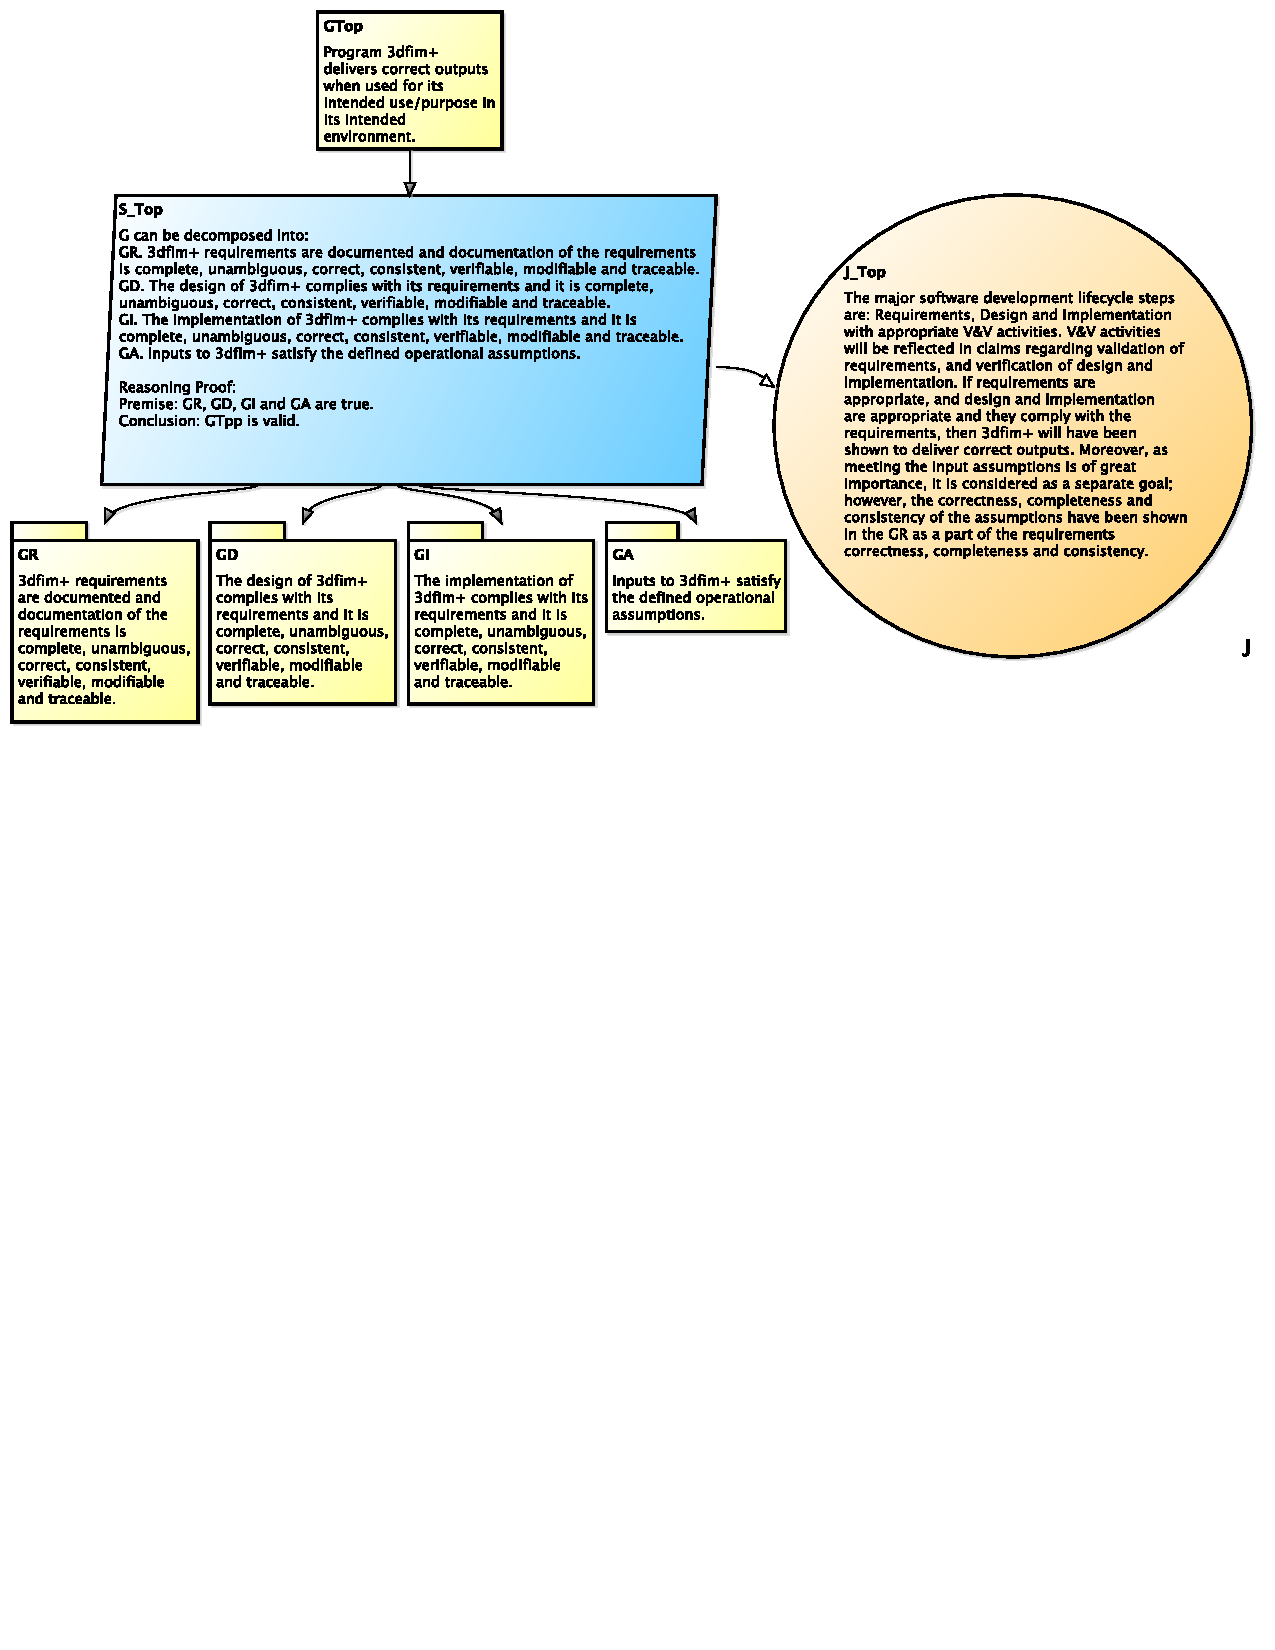
\includegraphics[width=1.15\textwidth]{../Figures/TopGoal.pdf}

\end{frame}
\hoffset=0in

%%%%%%%%%%%%%%%%%%%%%%%%%%%%%%%%%%%%%%%%%%%%%%%%%%%%%%%%%%%%%%%%%%%%%%%%%%%%%

\hoffset=-.2in
\begin{frame}[plain]
%\frametitle{GR Decomposition}

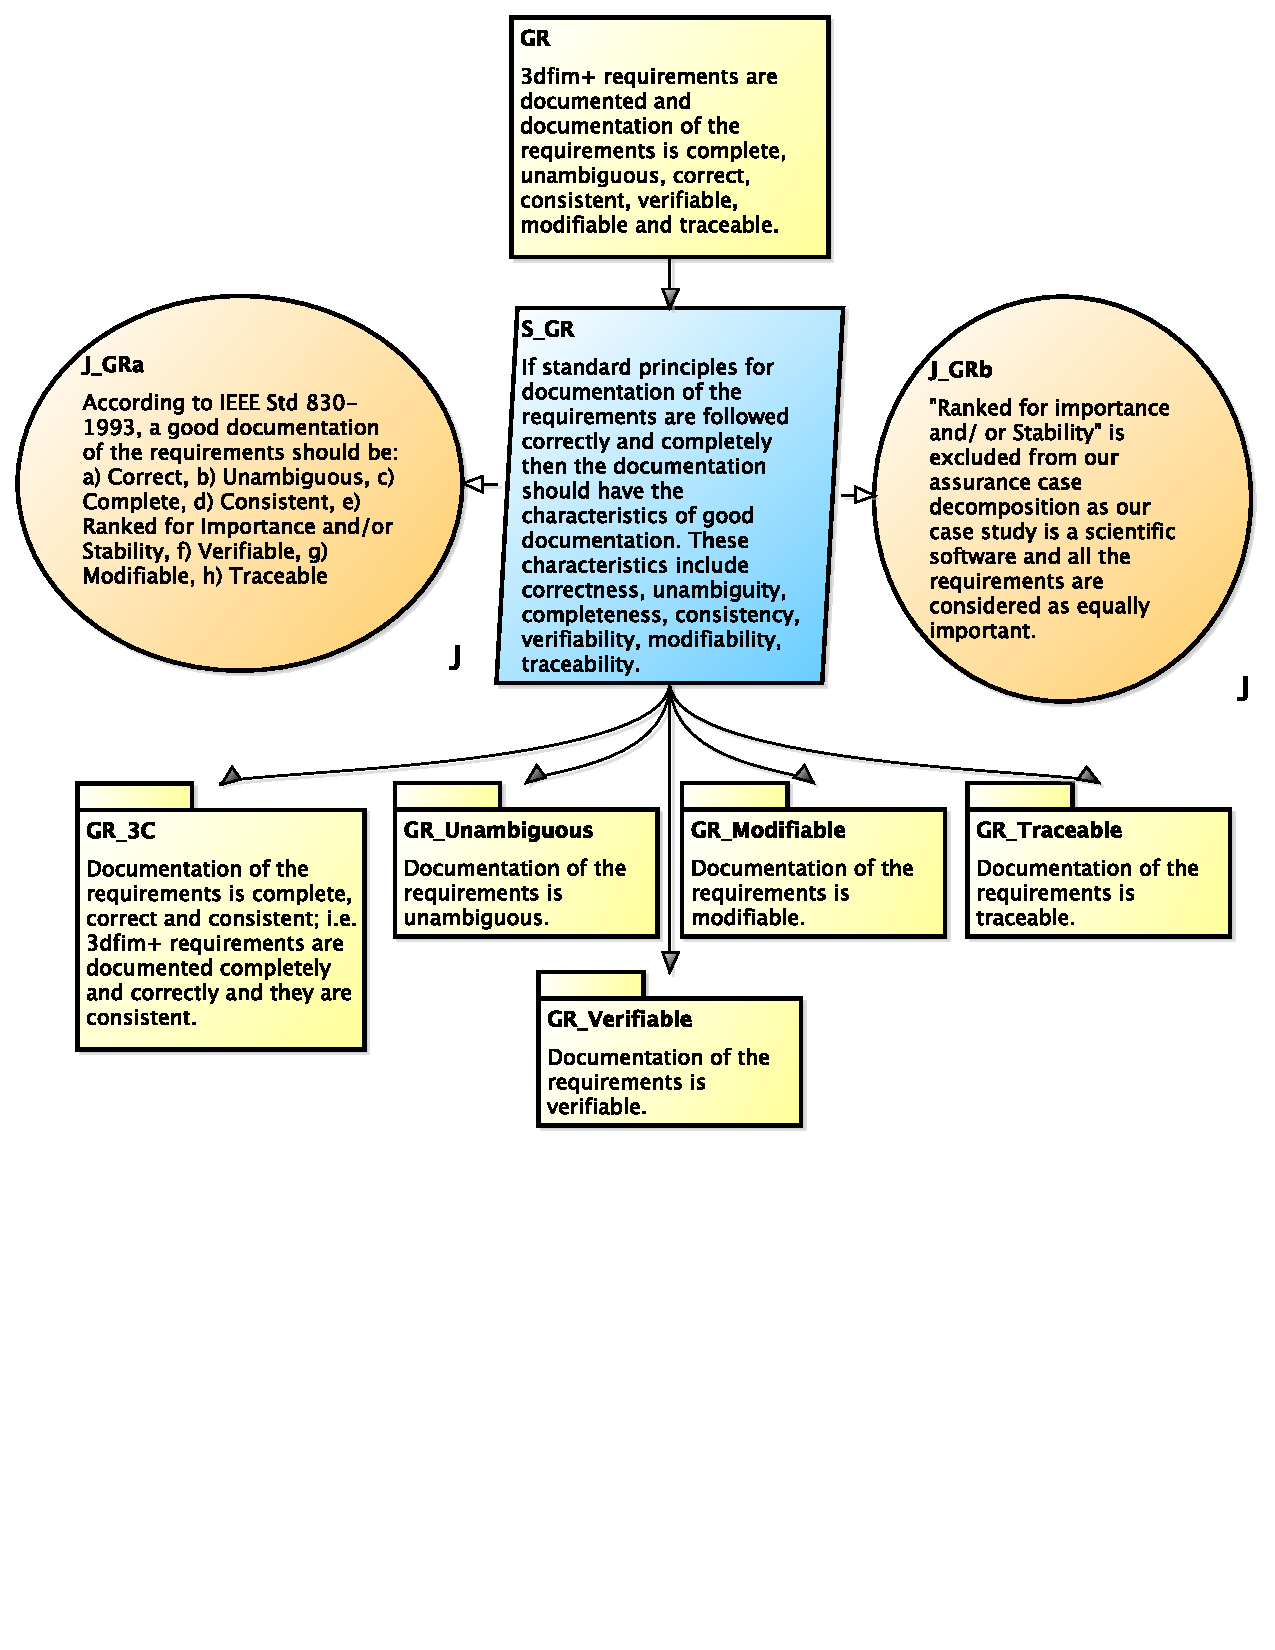
\includegraphics[width=0.95\textwidth]{../Figures/GRTop.pdf}

\end{frame}
\hoffset=0in

%%%%%%%%%%%%%%%%%%%%%%%%%%%%%%%%%%%%%%%%%%%%%%%%%%%%%%%%%%%%%%%%%%%%%%%%%%%%%

\hoffset=-.21in
\begin{frame}[plain]
%\frametitle{Modifiability of Documentation Requirements}

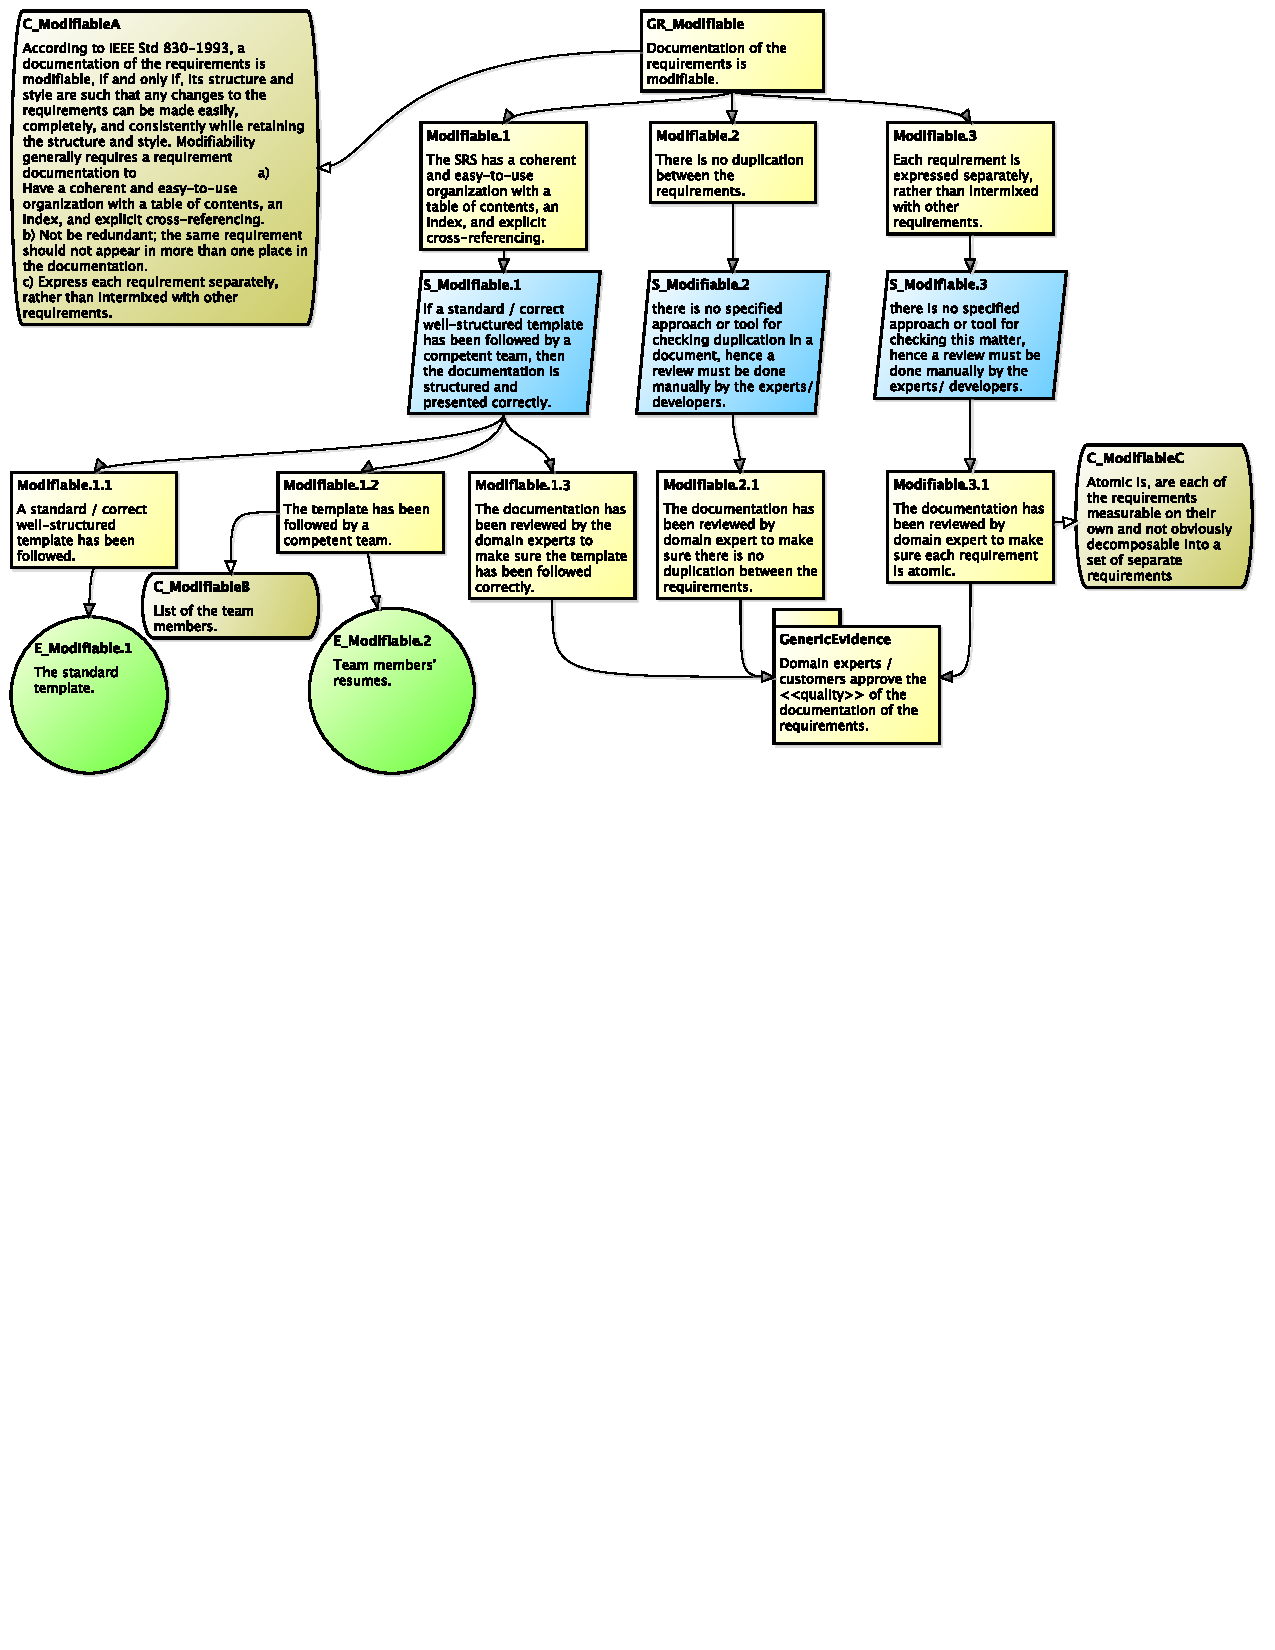
\includegraphics[width=1.14\textwidth]{../Figures/Modifiable.pdf}

\end{frame}
\hoffset=0in

%%%%%%%%%%%%%%%%%%%%%%%%%%%%%%%%%%%%%%%%%%%%%%%%%%%%%%%%%%%%%%%%%%%%%%%%%%%%%

\hoffset=-.3in
\begin{frame}[plain]
%\frametitle{Generic Evidence}

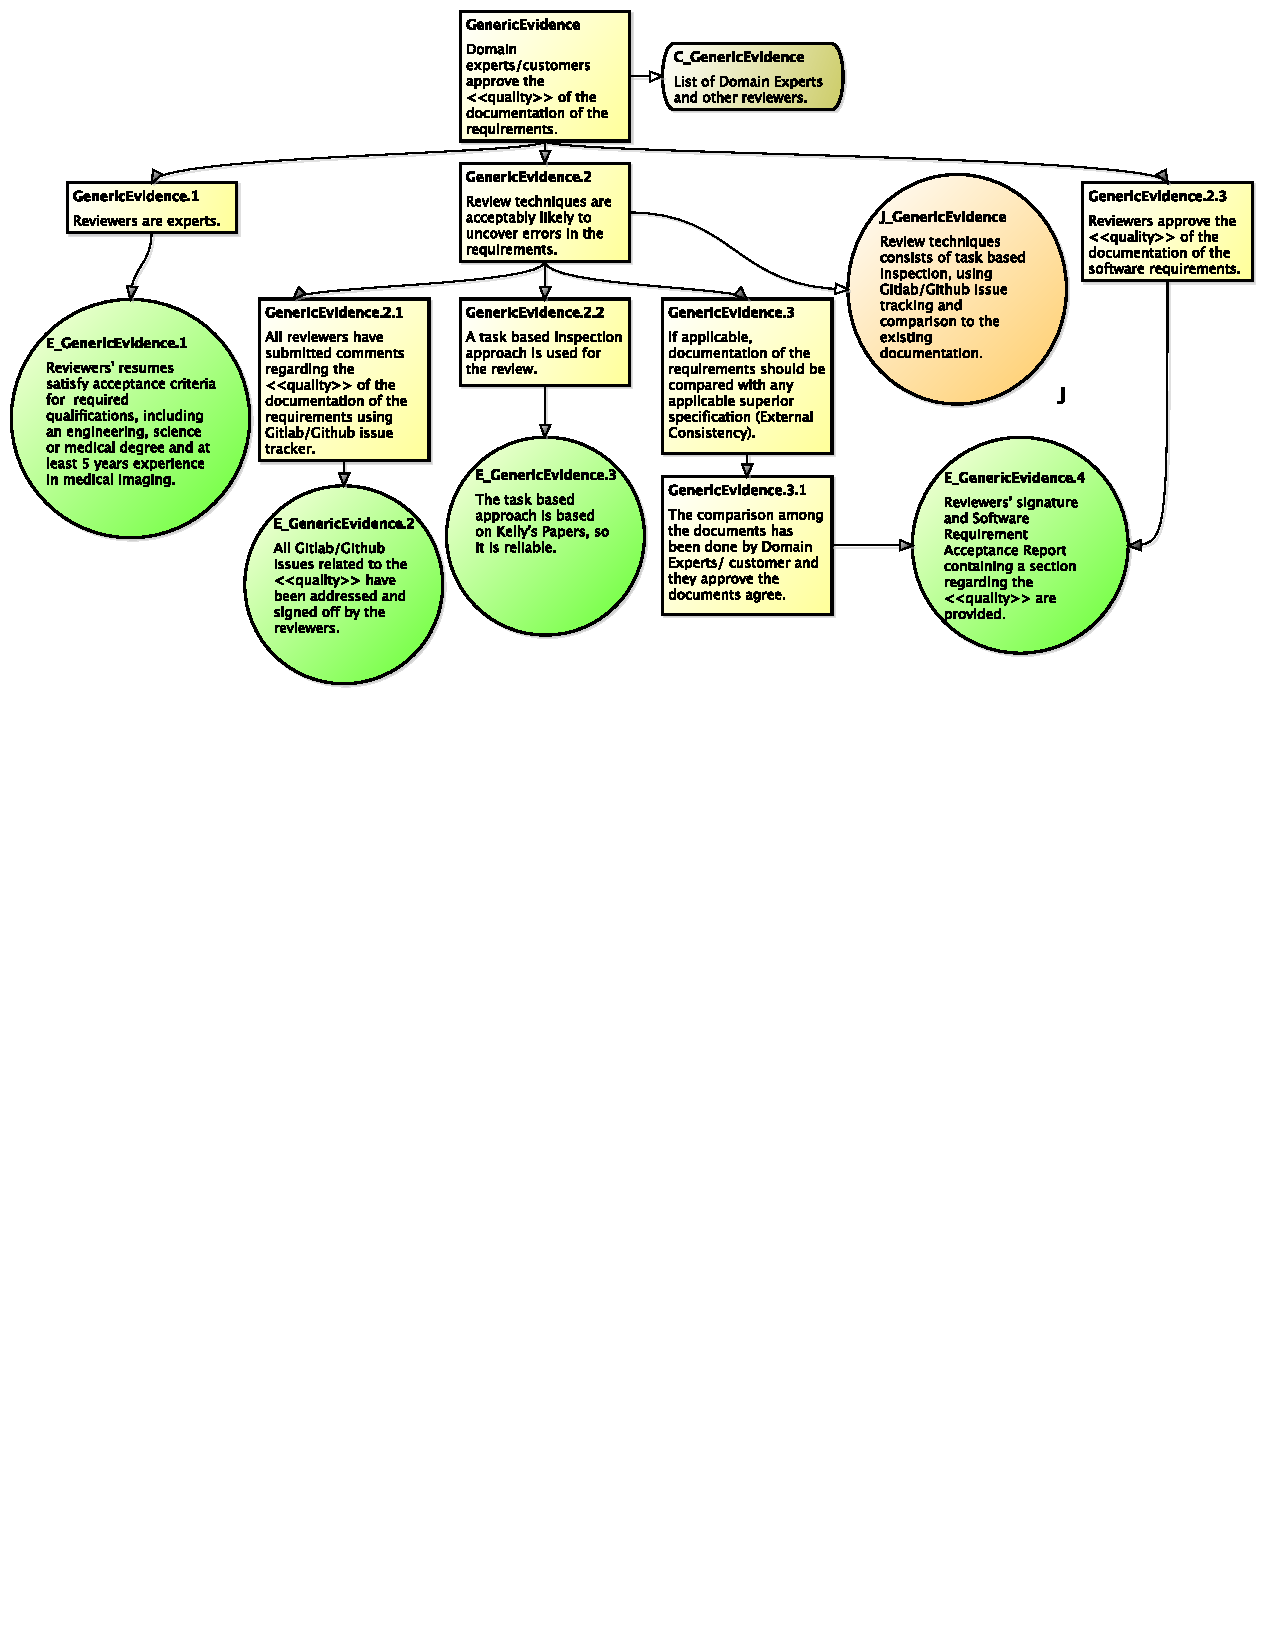
\includegraphics[width=1.15\textwidth]{../Figures/Generic.pdf}

\end{frame}
\hoffset=0in

%%%%%%%%%%%%%%%%%%%%%%%%%%%%%%%%%%%%%%%%%%%%%%%%%%%%%%%%%%%%%%%%%%%%%%%%%%%%%

\hoffset=-.2in
\begin{frame}[plain]
%\frametitle{Defined Operational Assumptions}

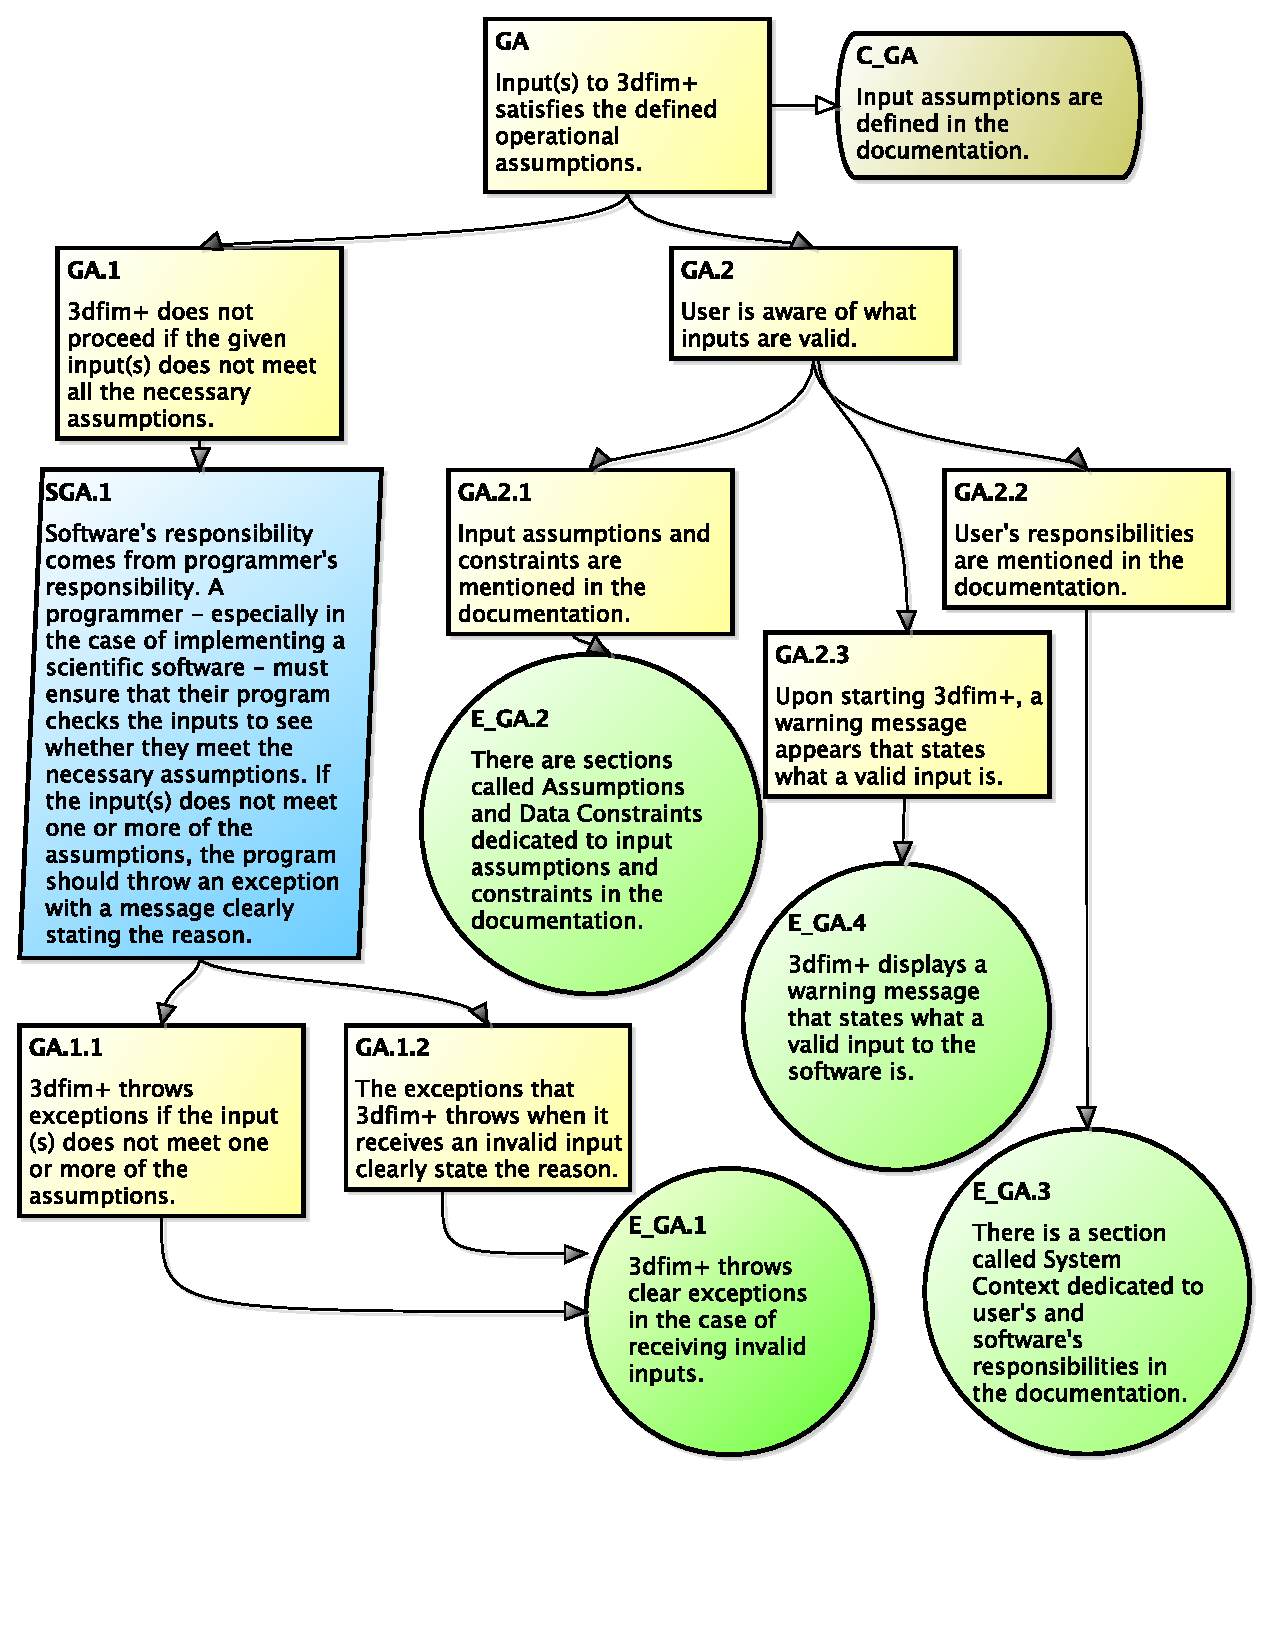
\includegraphics[width=0.75\textwidth]{../Figures/GSN_GA.pdf}

\end{frame}
\hoffset=0in

%%%%%%%%%%%%%%%%%%%%%%%%%%%%%%%%%%%%%%%%%%%%%%%%%%%%%%%%%%%%%%%%%%%%%%%%%%%%%

\begin{frame}
\frametitle{Proposed Changes to 3dfim+}

\bi
\item No mistakes found in calculations
\item Goal of original software was not certification
\item Problems found
\bi
\item GR goal not satisfied
\bi
\item Not complete, verifiable, modifiable or traceable
\item Coordinate system information missing
\item Ambiguous rank function
\ei
\item Inputs not checked in code
\item User not informed of their responsibility to use tool with correct
  statistical model
\ei
\ei

\end{frame}

%%%%%%%%%%%%%%%%%%%%%%%%%%%%%%%%%%%%%%%%%%%%%%%%%%%%%%%%%%%%%%%%%%%%%%%%%%%%%

\begin{frame}
\frametitle{Concluding Remarks}

\bi
\item Hopefully motivated assurance cases for SC
\item Quality is improved by looking at a problem from different perspectives,
  assurance cases provide a systematic and rigorous way to introduce a new
  perspective
\item An assurance cases will likely use the same documentation and ideas used
  in CAS 741
\item However, an assurance case can focus and direct efforts right from the
  start of the project
\ei

\end{frame}

%%%%%%%%%%%%%%%%%%%%%%%%%%%%%%%%%%%%%%%%%%%%%%%%%%%%%%%%%%%%%%%%%%%%%%%%%%%%%

\begin{frame}[allowframebreaks]
\frametitle{References}

\bibliography{../../ReferenceMaterial/References}

\end{frame}

%%%%%%%%%%%%%%%%%%%%%%%%%%%%%%%%%%%%%%%%%%%%%%%%%%%%%%

\end{document}